%! Author = Michał_Komputer
%! Date = 14.10.2021

% Preamble
\documentclass[a4paper,11pt]{article}

% Packages
\usepackage[polish]{babel}
\usepackage[T1]{fontenc}
\usepackage[utf8]{inputenc}
\usepackage{array}
\usepackage{enumerate}
\usepackage{float}
\usepackage{graphicx}
\usepackage{latexsym}
\usepackage{polski}
\usepackage{tabularx}
\usepackage[backend=bibtex,style=alphabetic]{biblatex}


% Title page
\title{Optymalizacja hiperparametrów procesu uczenia sieci neuronowych z wykorzystaniem algorytmu genetycznego}
\author{Michał Zawadzki}
\date{Czerwiec 2021}


% Additial settings
\DeclareUnicodeCharacter{266D}{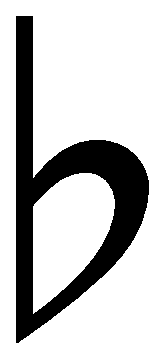
\includegraphics[height=1ex]{music_flat_sign}}
\DeclareUnicodeCharacter{266F}{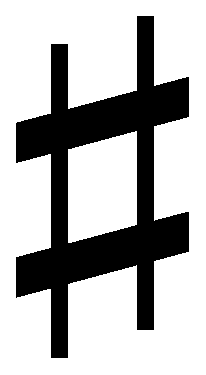
\includegraphics[height=1ex]{music_sharp_sign}}
\addbibresource{references.bib}
\restylefloat{table}

% Document
\begin{document}

    \maketitle

    \tableofcontents


    \section{Wstęp}

    \subsection{Cel pracy}
    Korzystając ze zbioru danych o utworach muzycznych dostępnych na platformie streaming-owej Spotify, stworzono kilka modeli szacujących jaką popularność osiągnie na tej platformie nowy utwór. Modele te są prostymi sieciami neuronowymi o różnej architekturze. Do optymalizacji ich hiperparametrów uczenia wykorzystano algorytm genetyczny.

    \subsection{Teza główna}
    Algorytm genetyczny może znacząco przyspieszyć proces wyboru optymalnych hiperparametrów uczenia dla wstępnie zaprojektowanej sieci neuronowej.


    \section{Wpływ cech utworów muzycznych na popularność}

    Zaczynając rozważania nad przyczynami, które sprawiają że niektóre utwory muzyczne osiągają ogromną popularność, podczas gdy inne nie zdobywają uznania szerokiego audytorium, trzeba najpierw zdefiniować podstawowe czynniki jakimi kieruje się odbiorca przy dokonywaniu wyborów muzycznych. Magdalena Parus-Jankowska i Szymon Nożyński w swojej pracy "Preferencje Muzyczne w Dobie Popularności Strumieniowego Słuchania Muzyki"\cite{PreferencjeMuzyczneWCzasachSteamingu2020} wymieniają 3 takie czynniki:
    \begin{itemize}
        \item \textit{upodobania} - Przywiązanie do konkretnych gatunków muzycznych, wraz z otaczającym je kontekstem kulturowym.
        \item \textit{smak/gust} - Umiejętność dostrzegania i oceny poszczególnych elementów składowych utworu, także znajomość i zrozumienie przesłania utworu.
        \item \textit{preferencje} - Upodobanie dla konkretnych utworów lub twórców muzycznych.
    \end{itemize}
    Czynniki te często kształtują się równolegle i przenikają semantycznie, dlatego też dla uproszczenia w dalszej części posłużono się szeroko rozumianym pojęciem preferencji muzycznych.

    \bigskip

    Preferencje muzyczne człowieka nie są czymś stałym. Zmieniają się one przez całe życie, szczególnie intensywnie w wieku dziecięcym i w okresie dojrzewania\cite{PreferencjeMuzyczneWCzasachSteamingu2020}.Wielki wpływ na sposób konsumpcji treści muzycznych ma środowisko, z którego człowiek się wywodzi, jego wykształcenie, zamożność, światopogląd i osobowość\cite{PreferencjeMuzyczneWCzasachSteamingu2020}. Muzyki słuchają najczęściej ludzie młodzi (w grupie wiekowej 18-24 lata 77\% deklarowało słuchanie muzyki codziennie\cite{cbos2018}) i to oni pośrednio, a bezpośrednio wywodzący się z tej grupy twórcy, kształtują nowe trendy i czynią rynek muzyczny bardzo dynamicznym.

    \bigskip

    Wejście na rynek serwisów streaming-owych, których sztandarowym przykładem jest szwedzki gigant Spotify, dokonało małej rewolucji na rynku muzycznym. Serwis działa w dwóch modelach płatności: bezpłatnym (z reklamami) i subskrypcyjnym. Można korzystać z niego za pośrednictwem przeglądarki, ale dostępne są także dedykowane aplikacje ma praktycznie każdą platformę, zaczynając od smart car-u na smartfonie kończąc, między którymi można się swobodnie przełączać. Muzyki można słuchać zarówno w trybie online, jak i w trybie offline (oczywiście po wcześniejszym pobraniu na urządzenie). Co ważne zmianie uległ sposób konsumpcji samych treści. Autor niniejszej pracy, jako szczególnie aktywny użytkownik serwisu (być może bardziej adekwatnym określeniem byłaby platforma) uznał za stosowne wymienienie następujących alternatywnych kanałów:
    \begin{itemize}
        \item \textit{strona główna (ang. home)} - Najmocniej promowane przez serwis treści, również spersonalizowane sekcje z dedykowanymi playlistami, a także szybki dostęp do treści ostatnio odtwarzanych.
        \item \textit{radio wykonawcy, radio utworu} - Pseudo-radio, a właściwie strumień muzyczny generowany przez algorytm Spotify dla danego wykonawcy lub konkretnego utworu muzycznego
        \item \textit{aktywność znajomych} - Trzeba nadmienić, że Spotify jest też serwisem społecznościowym. Mamy wgląd w bieżącą aktywność znajomych (o ile słuchają muzyki w trybie sesji publicznej).
        \item \textit{playlisty publiczne} - Playlisty stworzone przez pracowników serwisu, algorytmy oraz członków społeczności. Równolegle do klasycznego podziału na gatunki muzyczne, serwis proponuje także bardziej utylitarne kategorie, jak na przykład muzykę dobrą do ćwiczeń, czytania czy wyciszenia się przed snem.
        \item \textit{playlisty prywatne} - Playlisty stworzone przez użytkownika, nieupublicznione.
        \item \textit{biblioteka} - Treści pobrane przez użytkownika.
    \end{itemize}

    \bigskip

    Nie ulega wątpliwości, że wewnętrzna polityka serwisów muzycznych w zakresie promowania i pozycjonowania treści (w którą niestety nie ma wglądu, a która z ogromną dozą prawdopodobieństwa dyktowana jest przede wszystkim chęcią powiększania zasięgów i poprawy wyników finansowych) ma niebagatelny wpływ na wybory dokonywane przez użytkowników\cite{PreferencjeMuzyczneWCzasachSteamingu2020}. Zdaniem autora niniejszej pracy szczególnie duże znaczenie w tym aspekcie mają kryteria, na których oparty jest mechanizm wyszukiwania, a także (a może przede wszystkim) mechanizm dolosowywania kolejnych utworów w usłudze \textit{radio}. Z drugiej strony prawdziwe zdaje się być twierdzenie, że dobra muzyka obroni się sama. Bez względu na to jak bardzo konsument będzie zasypywany promowanymi treściami i tak regularnie będzie wracać tylko do tego co najbardziej trafiło w jego gusta, czy mówiąc bardziej górnolotnie (ale chyba w wielu przypadkach zasadnie) do jego duszy.

    \bigskip

    Christoph Dr{\"o}sser, popularny w Niemczech dziennikarz popularnonaukowy, napisał "Muzyka jest [\ldots] doświadczeniem całościowym, w znacznym stopniu nierozsądnym, którego nie da się ogarnąć za pomocą zimnego, racjonalnego instrumentarium nauki"\cite{MuzykaDajSieUwiesc2021}. Ale czy to aby na pewno prawda? Na początku 20-go wieku w mainstreamie zaczęło funkcjonować pojęcie \textit{Hit Song Science} (pl. nauka o przebojach muzycznych), za którego twórcę i głównego promotora uważa się Mike'a McCready\cite{HitSongScienceWiki}. McCready wraz ze współpracownikami, działając w ramach firmy Polyphonic HMI, starał się rozwijać i sprzedawać wytwórniom muzycznym narzędzia, oparte o techniki \textit{MIR} (music information retrieval, pl. pozyskiwanie informacji muzycznych z utworu) i \textit{data science}, ułatwiające przewidywanie czy dany utwór ma szanse stać się 'hitem'\cite{PolyphonicHMIWiki}. Odnośnie podstaw naukowych \textit{Hit Song Science} od lat, w szczególności w społeczności \textit{MIR}, toczy się burzliwa, nie rozstrzygnięta do końca debata\cite{HitSongScienceWiki}.

    \bigskip

    François Pachet i Pierre Roy z firmy Sony Computer Science Laboratories, Inc. w artykule "Hit Song Science Is Not Yet a Science" z 2009-go roku\cite{HitSongScienceNotYet2009} opisują swoją nieudaną próbę stworzenia klasyfikatora szacującego popularność utworów muzycznych na podstawie ich cech muzycznych oraz subiektywnych "ludzkich" etykiet przypisanych przez profesjonalnych ankieterów. Danymi, na których pracowali była baza 32978 dostarczona przez firmę HiFind. W swoim ekperymencie oprócz zaawansowanych technik \textit{MIR} wykorzystali oni \textit{Support Vector Machine} (pl. maszyna wektorów nośnych). Wyniki uzykane dla poszczególnych prób tylko nieznacznie różniły się od losowych. Za przyczynę niepowodzenia uznano niewłaściwy dobór zestawu parametrów użytych do stworzenia modelu.

    \bigskip

    O wiele bardziej obiecujące wyniki uzyskali Yizhao Ni, Ra´ul Santos-Rodr´ıguez, Matt Mcvicar i Tijl De Bie z kooperacji uniwersytetów University of Bristol i Universidad Carlos III de Madrid. W swoim artykule "Hit Song Science Once Again a Science?" z 2011-go roku\cite{HitSongScienceOnceAgain2011} (już poprzez sam tytuł ustawiając się w kontrapunkcie do poprzedników) przedstawiają wyniki swojego eksperymentu przeprowadzonego na zbiorze 5947 utworów z brytyjkiej listy przebojów z lat 1960-2010. Do ekstrakcji wartości paramerów muzycznych wykorzystali oni narzędzie EchoNest. Jako model wykorzystani oni prosty ruchomy percepron (ang. \textit{Shifting perceptron}) będący funkcją czasu. Wyniki eksperymentów tym razem różniły się znacząco na korzyść w porównaniu do odczytów losowych. Badaczom udało się też sformułować na ich podstawie szereg cennych wniosków.

    \bigskip
    Wychodząc z założenia, że na przestrzeni ostatniej dekady nastąpił ogromy postęp w dziedzinie data science, w szczególności w obszarze badań nad głębokami sieciami neuronowymi, a także (co nie mniej istotne) dostępne są ogromne bazy zawierające wysokiej jakości, świetnie ustandaryzowane i udokumentowane dane udostępnioe przez serwisy muzyczne takie jak Spotify, autor niniejszej pracy z dużym entuzjazmem postanowił podjąć się samodzielnej próby stworzenia wysokiej klasy modelu do predykcji popularności utworów muzycznych.


    \section{Sieci neuronowe}


    \section{Algorytmy Genetyczne}


    \section{Zastosowanie dwustopniowego algorytmu uczenia maszynowego do predykcji popularności utworu}


    \section{Opis zbioru danych}

    Zbiór danych zawiera informacje o ponad 170 tysiącach utworów muzycznych, opublikowanych w latach 1921-2020 i dostępnych na szwedzkiej platformie streaming-owej Spotify. Dataset został stworzony przy wykorzystaniu oficjalnego, publicznego API deweloperskiego Spotify i udostępniony na platformie Kaggle w formacie CSV przez użytkownika Yamaç Eren Ay.

    \bigskip

    Oryginalny dataset to zbiór tabelaryczny zawierający 170653 rekordów podzielonych na 19 kolumn. Kolumny te to kolejno:
    \begin{itemize}
        \item \textit{valence} (pl.ozdobnik) - Miara w skali od 0.0 do 1.0 określająca stopień 'pozytywności' przekazywany przez utwór. Utwory z wysoką wartością współczynnika \textit{valence} brzmią bardziej pozytywnie (szczęśliwie, radośnie lub euforycznie), podczas gdy niska wartość tego współczynnika objawia się brzmieniem negatywnym (smutnym, depresyjnym, zdenerwowanym lub wściekłym).
        \item \textit{year} (pl. rok) - Rok publikacji utwory. Wartości między 1921 a 2020 włącznie.
        \item \textit{acousticness} (pl. akustyczność) - Miara w skali od 0.0 do 1.0 określająca pewność, z jaką dany utwór można zakwalifikować jako akustyczny. 1.0 - wskazuje na wysoką pewność, 0.0 na bardzo niską.
        \item \textit{artists} (pl. artyści) - Lista imion i nazwisk lub pseudonimów artystycznych artystów wykonujących dany utwór.
        \item \textit{danceability} (pl. taneczność) - Miara w skali od 0.0 do 1.0 określająca, w jakim stopniu dany utwór jest odpowiedni do tańca, wyliczana jako kombinacja takich parametrów muzycznych ja tempo, stabilność rytmu, moc taktu i ogólna regularność. 1.0 oznacza wysoką taneczność, a 0.0 - bardzo niską.
        \item \textit{duration\_ms} (pl. czas trwania) - Czas trwania utworu w milisekundach.
        \item \textit{energy} (pl. energia) - Miara w skali od 0.0 do 1.0 reprezentująca odczuwalny stopień intensywności i aktywności utworu. Typowy utwory 'energetyczne' są odbierane jako szybkie, głośne czy wręcz hałaśliwe. Przykładem wysokiej energetyczności mogą byś utwory death-metalowe, podczas gdy preludia Bacha będą cechowały się niską energetycznością. Postrzegalne czynniki wpływające na tą cechę to dynamiczny zakres, odbierana głośność, tembr, \textit{onset rate} (pl. współczynnik rozpoczęć ??) i ogólna entropia.
        \item \textit{explicit} (pl. odważny, śmiały) - Wartość \textit{true} (pl. prawda)/\textit{false} (pl. fałsz). Flaga określająca czy dany utwór zawiera wulgaryzmy, treści erotyczne, treści nacechowane przemocą, wzmianki o nielegalny używkach i tym podobne; w ogólności treści skierowane do odbiorców pełnoletnich.
        \item \textit{id} (pl. identyfikator) - Unikalne, alfanumeryczne Spotify ID dla utworu.
        \item \textit{instrumentalness} (pl. instrumentalność) - Miara prawdopodobieństwa określająca, czy dany utwór nie zawiera wstawek wokalnych (fragmentów śpiewanych). Wyrazy dźwiękonaśladowcze takie jak 'ooh' czy 'aah' przez algorytm/klasyfikator są traktowane jako instrumentalne. Rap czy zwykła mowa traktowana jako 'czysty wokal'. In bliżej wartości parametru \textit{instrumentalness} do wartości 1.0, tym wyższe prawdopodobieństwo braku wokali. Wartości powyżej 0.5 w założeniu mają reprezentować utwory instrumentalne, natomiast prawdopodobieństwo prawidłowej klasyfikacji rośnie wraz ze zbliżaniem się wskaźnika do wartości 1.0.
        \item \textit{key} (pl. tonacja). Tonacja utworu przedstawiona jako liczba całkowita nieujemna: 0,1,2\ldots . Liczby zmapowane są na standardową notację muzyczną: 0 = C, 1 = C♯/D♭, 2 = D i tak dalej.
        \item \textit{liveness} - (pl. żywość, żywiołowość) - Miara żywiołowości określa prawdopodobieństwo obecność publiczności podczas nagrania. Wartości \textit{liveness} powyżej 0.8 wskazują na wysokie prawdopodobieństwo, że utwór wykonywany był 'na żywo'.
        \item \textit{loudness} (pl. głośność) - Ogólna głośność utworu mierzona w decybelach. Wartości głośności są wyliczane poprzez uśrednienie głośności całego utworu, co sprawia, że metryka staje się użyteczna do porównywania utworów. Głośność jest cechą dźwięku ściśle skorelowaną z amplitudą fali dźwiękowej. Wartości w większości przypadków wahają się między -60 a 0 db.
        \item \textit{mode} (pl. tryb, dominanta) - Parametr 'mode' oznacza modalność utworu: \textit{major} (pl. główna, pierwszorzędna) lub \textit{minor} (pl. pomniejsza, drugorzędna), w znaczeniu typu skali, w której znajduje się warstwa melodyczna. 1 oznacza \textit{major}, 0 to \textit{minor}.
        \item \textit{name} (pl. nazwa) - Tytuł piosenki, utworu lub nagrania.
        \item \textit{popularity} (pl. popularność) - Popularność utworu w skali od 0 do 100, gdzie 100 oznacza najwyższą popularność. Popularność wyliczana jest przez algorytm, bazujący przede wszystkim na liczbie odtworzeń utworu, ale także na tym jak świeże (odległe od chwili obecnej) są te odtworzenia.
        \item \textit{release\_date} (pl. data publikacji) - Data publikacji utworu lub albumu, na którym znalazł się utwór.
        \item \textit{speechiness} (pl. wypełnienie mową) - Parametr \textit{speechiness} określa stopień obecności mowy w utworze. Nagrania wypełnione mową takie jak programy 'talk show', audiobooki czy poematy będą uzyskiwały wartości tego parametru zbliżone do 1.0. Wartości powyżej 0.66 wskazują na wysokie prawdopodobieństwo wypełnienia nagrania w całości mową. Wartości od 0.33 do 0.66 wskazują na występowanie zarówno mowy jak i muzyki, zarówno w następujących po sobie sekwencjach, jak i w nakładających się na siebie warstwach dźwiękowych. Wartości poniżej 0.33 oznaczają duże prawdopodobieństwo nie występowania mowy w utworze.
        \item \textit{tempo} (pl. tempo) - Ogólne szacowane tempo utworu w taktach na minutę (ang. \textit{BPM}). W terminologi muzycznej, tempo jest szybkością danego fragmentu/kawałka utworu wyliczaną bezpośrednio w oparciu o średnią długość taktu.
    \end{itemize}
    Opisy parametrów są luźnym tłumaczeniem oficjalnej dokumentacji API deweloperskiego Spotify\cite{SpotifyWebAPIReference}.

    \bigskip

    Do stworzenia modeli wykorzystano następujące parametry: \textit{valence}, \textit{acousticness}, \textit{danceability}, \textit{duration\_ms}, \textit{energy}, \textit{explicit}, \textit{instrumentalness}, \textit{key}, \textit{liveness}, \textit{loudness}, \textit{mode}, \textit{release\_date}, \textit{speechiness} i \textit{tempo} Trzeba tu nadmienić, że na potrzeby dalszych działań wartości parametru \textit{key} zostały zamienione na binarną postać wektorową (ang. \textit{one-hot encoding}), a wartości \textit{release\_date} na milisekundy w standardzie UNIX. Na podstawie wartości wcześniej wymienionych parametrów modele szacowały wartość popularności (ang. \textit{popularity}) utworu.


    \section{Rezultaty eksperymentów}


    \section{Wnioski}

    \nocite{*}
    \printbibliography
\end{document}